\documentclass[12pt]{article}

%%%%%%%%%%%%%%%%%%%%%%%%%%%%%%%%%%%%%%%%%%%%%%%%%%%%%%%%%%%%%%%%%%%%%%
%\pdfminorversion=4
% NOTE: To produce blinded version, replace "0" with "1" below.
%\newcommand{\blind}{0}

%%%%%%% IISE Transactions margin specifications %%%%%%%%%%%%%%%%%%%


\newcommand{\chartercomment}[1]{\begin{tcolorbox}[colback=yellow!10!white,
                    colframe=white!20!black,
                    title=\textsc{Charter of Turin guidelines},
                    center, 
                    valign=top, 
                    halign=left,
                    before skip=0.8cm, 
                    after skip=0.3cm,
                    center title, 
                    width=14cm]
    #1
\end{tcolorbox}}

\newcommand{\taskcomment}[1]{\begin{tcolorbox}[sharpish corners,
                    boxrule = 0pt,
                    toprule = 4.5pt,
                    center,
                    enhanced,
                    fuzzy shadow = {0pt}{-2pt}{-0.5pt}{0.5pt}{black!35}]
    #1
\end{tcolorbox}}

\newcommand{\taskdiagram}[1]{\href{#1}{
\includegraphics[width=50px]{logos/diagram}}}

\newcommand{\taskvideo}[1]{\href{#1}{
\includegraphics[width=50px]{logos/video}}}

\makeatother
%%%%%%%%%%%%%%%%%%%%%%%%%%%%%%%%%%%%%%%%%%%%%%%%%%%%%%%%%%%%%%%%%%%%%%%%%

%%%%% IISE Transactions package list %%%%%%%%%%%%%%%%%%%%%%%%%%%%%%%%%%%%%%
%\usepackage[toc,page]{appendix}
\usepackage[a4paper, margin=0.8in]{geometry}
\usepackage[toc,page]{appendix}
\usepackage{float}
\usepackage{setspace}
\usepackage{parskip}
\usepackage[bookmarks=false]{hyperref}
\usepackage{multicol}
\usepackage{amsmath}
\usepackage{graphicx}
\usepackage{enumerate}
\usepackage[many]{tcolorbox}
\usepackage{xcolor}
\usepackage{url}
\usepackage{caption}
\usepackage{pdflscape}
\usepackage[contents={}]{background}
\usepackage{tikz}
%%%%%%%%%%%%%%%%%%%%%%%%%%%%%%%%%%%%%%%%%%%%%%%%%%%%%%%%%%%%%%%%%%%%%%%

%%%%% Author package list and commands %%%%%%%%%%%%%%%%%%%%%%%%%%%%%%%%%%%%%%%%%%%%%
%%%%% Here are some examples %%%%%%%%%%%%%%
%	\usepackage{amsfonts, amsthm, latexsym, amssymb}
%	\usepackage{lineno}
%	\newcommand{\mb}{\mathbf}
%%%%%%%%%%%%%%%%%%%%%%%%%%%%%%%%%%%%%%%%%%%%%%%%%%%%%%%%%%%%%%%%%%%%%%%%%%%%%%
\hypersetup{colorlinks, linkcolor=blue, citecolor=blue, urlcolor=blue}
\graphicspath{{./images/}}
\addtocontents{toc}{\protect\setcounter{tocdepth}{1}}
	
\begin{document}
\include{document}
%\def\testee{restoration_repair_paint_complete}
\newpage
\setlength{\parindent}{0.25in}
%\appendix

\section{Charter of Turin}
\label{sec:charter_of_turin}

This document was produced by the Turin Charter Working Group / FIVA Cultural Commission (Thomas Kohler, Gundula Tutt, Rainer Hindrischedt, Mario De Rosa, Alfieri Maserati, Stefan Musfeld \& Mark Gessler). Its original version can be found online in FIVA's site\footnote{FIVA's Charter of Turin, \url{https://fiva.org/download/charter-of-turin-english-french/}}, both in English and French.


\subsection{Introduction}

The Fédération Internationale des Véhicules Anciens (FIVA) is the world federation of historic vehicle clubs. It supports and encourages the preservation and responsible use of historic vehicles as an important part of our technical and cultural heritage.

Historic vehicles are significant in their role as means of transport, as witnesses to their historic origins, the technical state of the art of their period and last but not least for their impact on society.

The scope of this Charter includes mechanically propelled road and nonrail land vehicles. A vehicle is considered to be historic once it complies with the Charter and the applicable FIVA definitions.

The Charter may also include buildings and related artefacts to historic vehicles and their period of operation, such as factories, fuel stations, roads or racetracks.

For many years the owners of historic vehicles, the curators of historic vehicle collections and the restorers of historic vehicles have been very successful at salvaging, preserving and keeping historic vehicles in operation.

This Charter was approved by FIVA to provide guidance for decisions and treatments in relation to historic vehicles. The Turin Charter unites the guiding principles for the use, upkeep, conservation, restoration and repair of historic vehicles.

This Charter is based on and inspired by UNESCO’s Venice Charter (1964), the Barcelona Charter (2003, historic ships) and the Riga Charter (2005, historic rail vehicles). 


\subsection{Articles}

\subsubsection{Article 1: Aim}

The aim of this Charter is to preserve and safeguard the history of vehicles including their engineering, form, functions and documented histories and their many and diverse relationships with society and social environments.

To understand, appreciate and ensure the preservation and operation of historic vehicles, including their use on public roads, it is important to use the research methods, scientific, historical and technical knowledge available and involve the organisations and facilities working in this sector.


\subsubsection{Article 2: Future}

Preservation, restoration and any related work processes are aimed at sustaining historic vehicles as both technical artefacts and witnesses of transport history and culture. It is imperative to pass on the methods used, material knowledge and work processes to future generations. We also aim to preserve the special knowledge, expertise and skills related to the manufacture and operation of such vehicles.


\subsubsection{Article 3: Care}

Permanent and sustainable care are essential for the survival of historic vehicles. Use of historic vehicles, including on public roads, is important for their preservation. It is the only way to fully understand and pass on the traditional knowledge of driving and maintaining them for future generations.


\subsubsection{Article 4: Position}

It is beneficial for the preservation of historic vehicles that they are seen as an integral part of public life and perceived as a contribution to our cultural heritage.

It is important and desirable that they can be used. However, in order to use them, historic vehicles should not be modified more than necessary. Unavoidable modifications should not interfere with the historic substance. As a matter of principle, they should not alter the vehicle’s period engineering and appearance.


\subsubsection{Article 5: Processes}

The preservation of historic vehicles can require interventions or restorations to different extents.

Preservation means the care and prevention from deterioration or damage, by which the present condition, individual and memorial quality of a historic vehicle or object is safeguarded.

Conservation includes all acts serving to secure and stabilise the vehicle or object that do not alter the historic substance, parts and materials. Conservation treatment will not put at risk the object’s historical or material documentary value in any way. It serves exclusively to prevent or at least delay continued deterioration. Usually, such measures are not visible on the surface.

Restoration is the process of replacing missing parts or areas with the aim of displaying an earlier state of the vehicle and goes further than conservation. Restored areas should discreetly blend in with the existing historic stock, but remain distinguishable on closer inspection. This is different from repair, that stands for the adaptation, refurbishment or replacement of existing or missing components. Repair makes a vehicle fully operational again and may not take into account the authentic substance belonging to the vehicle.

Preservation, conservation, and restoration are specialised processes aimed at safeguarding and displaying a vehicle’s engineering, aesthetic, functional, social and historic value. They should aim at understanding and considering the original design and the historic background of the individual vehicle. They should be based on respect for the individual historic entity and information found in authentic documents.


\subsubsection{Article 6: History}

Any changes and modifications to a vehicle which occurred during its ordinary life span and altering its condition as originally delivered are testimonials of the vehicle’s history and should be preserved as such. Therefore it is not necessary to restore a historic vehicle in a way that adjusts its look and technical features back to the appearance of the manufacturing date.

A restoration that would return a vehicle to the appearance of a certain period should only be attempted with careful examination of historical records  or thorough planning.

Components and materials inserted to replace historic parts in the process of a restoration should be identified with simple and permanent markings to distinguish them from the historic substance.

For replaced parts, FIVA recommends the marking system attached to this charter (see Appendix 1) 


\subsubsection{Article 7: Accuracy}

During the restoration of historic vehicles historically accurate materials and work techniques should be preferred, unless such materials or techniques can no longer be used because of safety concerns, lack of availability or legal prohibitions.

Especially in the conservation of historic substance, traditional materials may not be adequate. As elsewhere in the field of restoration, modern materials and working techniques may then be used instead, provided they have been proven adequate and durable in experiments or tried in practice.


\subsubsection{Article 8: Appearance}

Any modifications to a historic vehicle required outside of its ordinary lifespan should be integrated discreetly and respect the original structure and appearance.

Such modifications should be reversible. It is recommended that any important original parts removed should be kept with the vehicle for later use and to serve as reference of their original existence and make. 


\subsubsection{Article 9: Planning}

Any work undertaken on a historic vehicle should be planned systematically and documented in an appropriate manner. These records should be maintained with the vehicle. 


\subsubsection{Article 10: Archives}

Any persons, facilities and organisations involved in the preservation, conservation, restoration, repair and operation of historic vehicles should take appropriate steps to protect their records and archives.


\subsubsection{Article 11: Status}

Institutions engaged in the preservation and transfer of knowledge or specialist skills required in the preservation and operation of historic vehicles should seek recognition by international and national governmental authorities as cultural heritage institutions.

Archives consisting of documents, drawings, photographs or other media and artefacts relating to historic vehicles should be cared for as part of the cultural heritage. 


\subsection*{Appendix 1: Proposed marking system}

The system uses the following letters for permanent marking:

\begin{table}[H]
    \begin{tabular}{|l|l|p{7.2cm}|}
    \hline
    MARKERS & MEANING                      & DESCRIPTION\\
    \hline
    NB      & Newly Built                  & An accurate as possible a copy in terms of form, materials and make, reproduced directly from a documented original.\\ 
    \hline
    FR      & Free Reconstruction          & Reconstruction without using any historic model in terms of form, material or work technique. The part however fulfils the technical function of an historic component utilised earlier.\\
    \hline
    CS      & Conservational Stabilisation & A later structural reinforcement added to stabilize the historic substance.\\ \hline
    \end{tabular}
\end{table}

We recommend the indication of the year of restoration/manufacture of the replacement part with the two-letter code.


\newpage
  
\backgroundsetup{
  scale=1,
  angle=0,
  opacity=1,
  contents={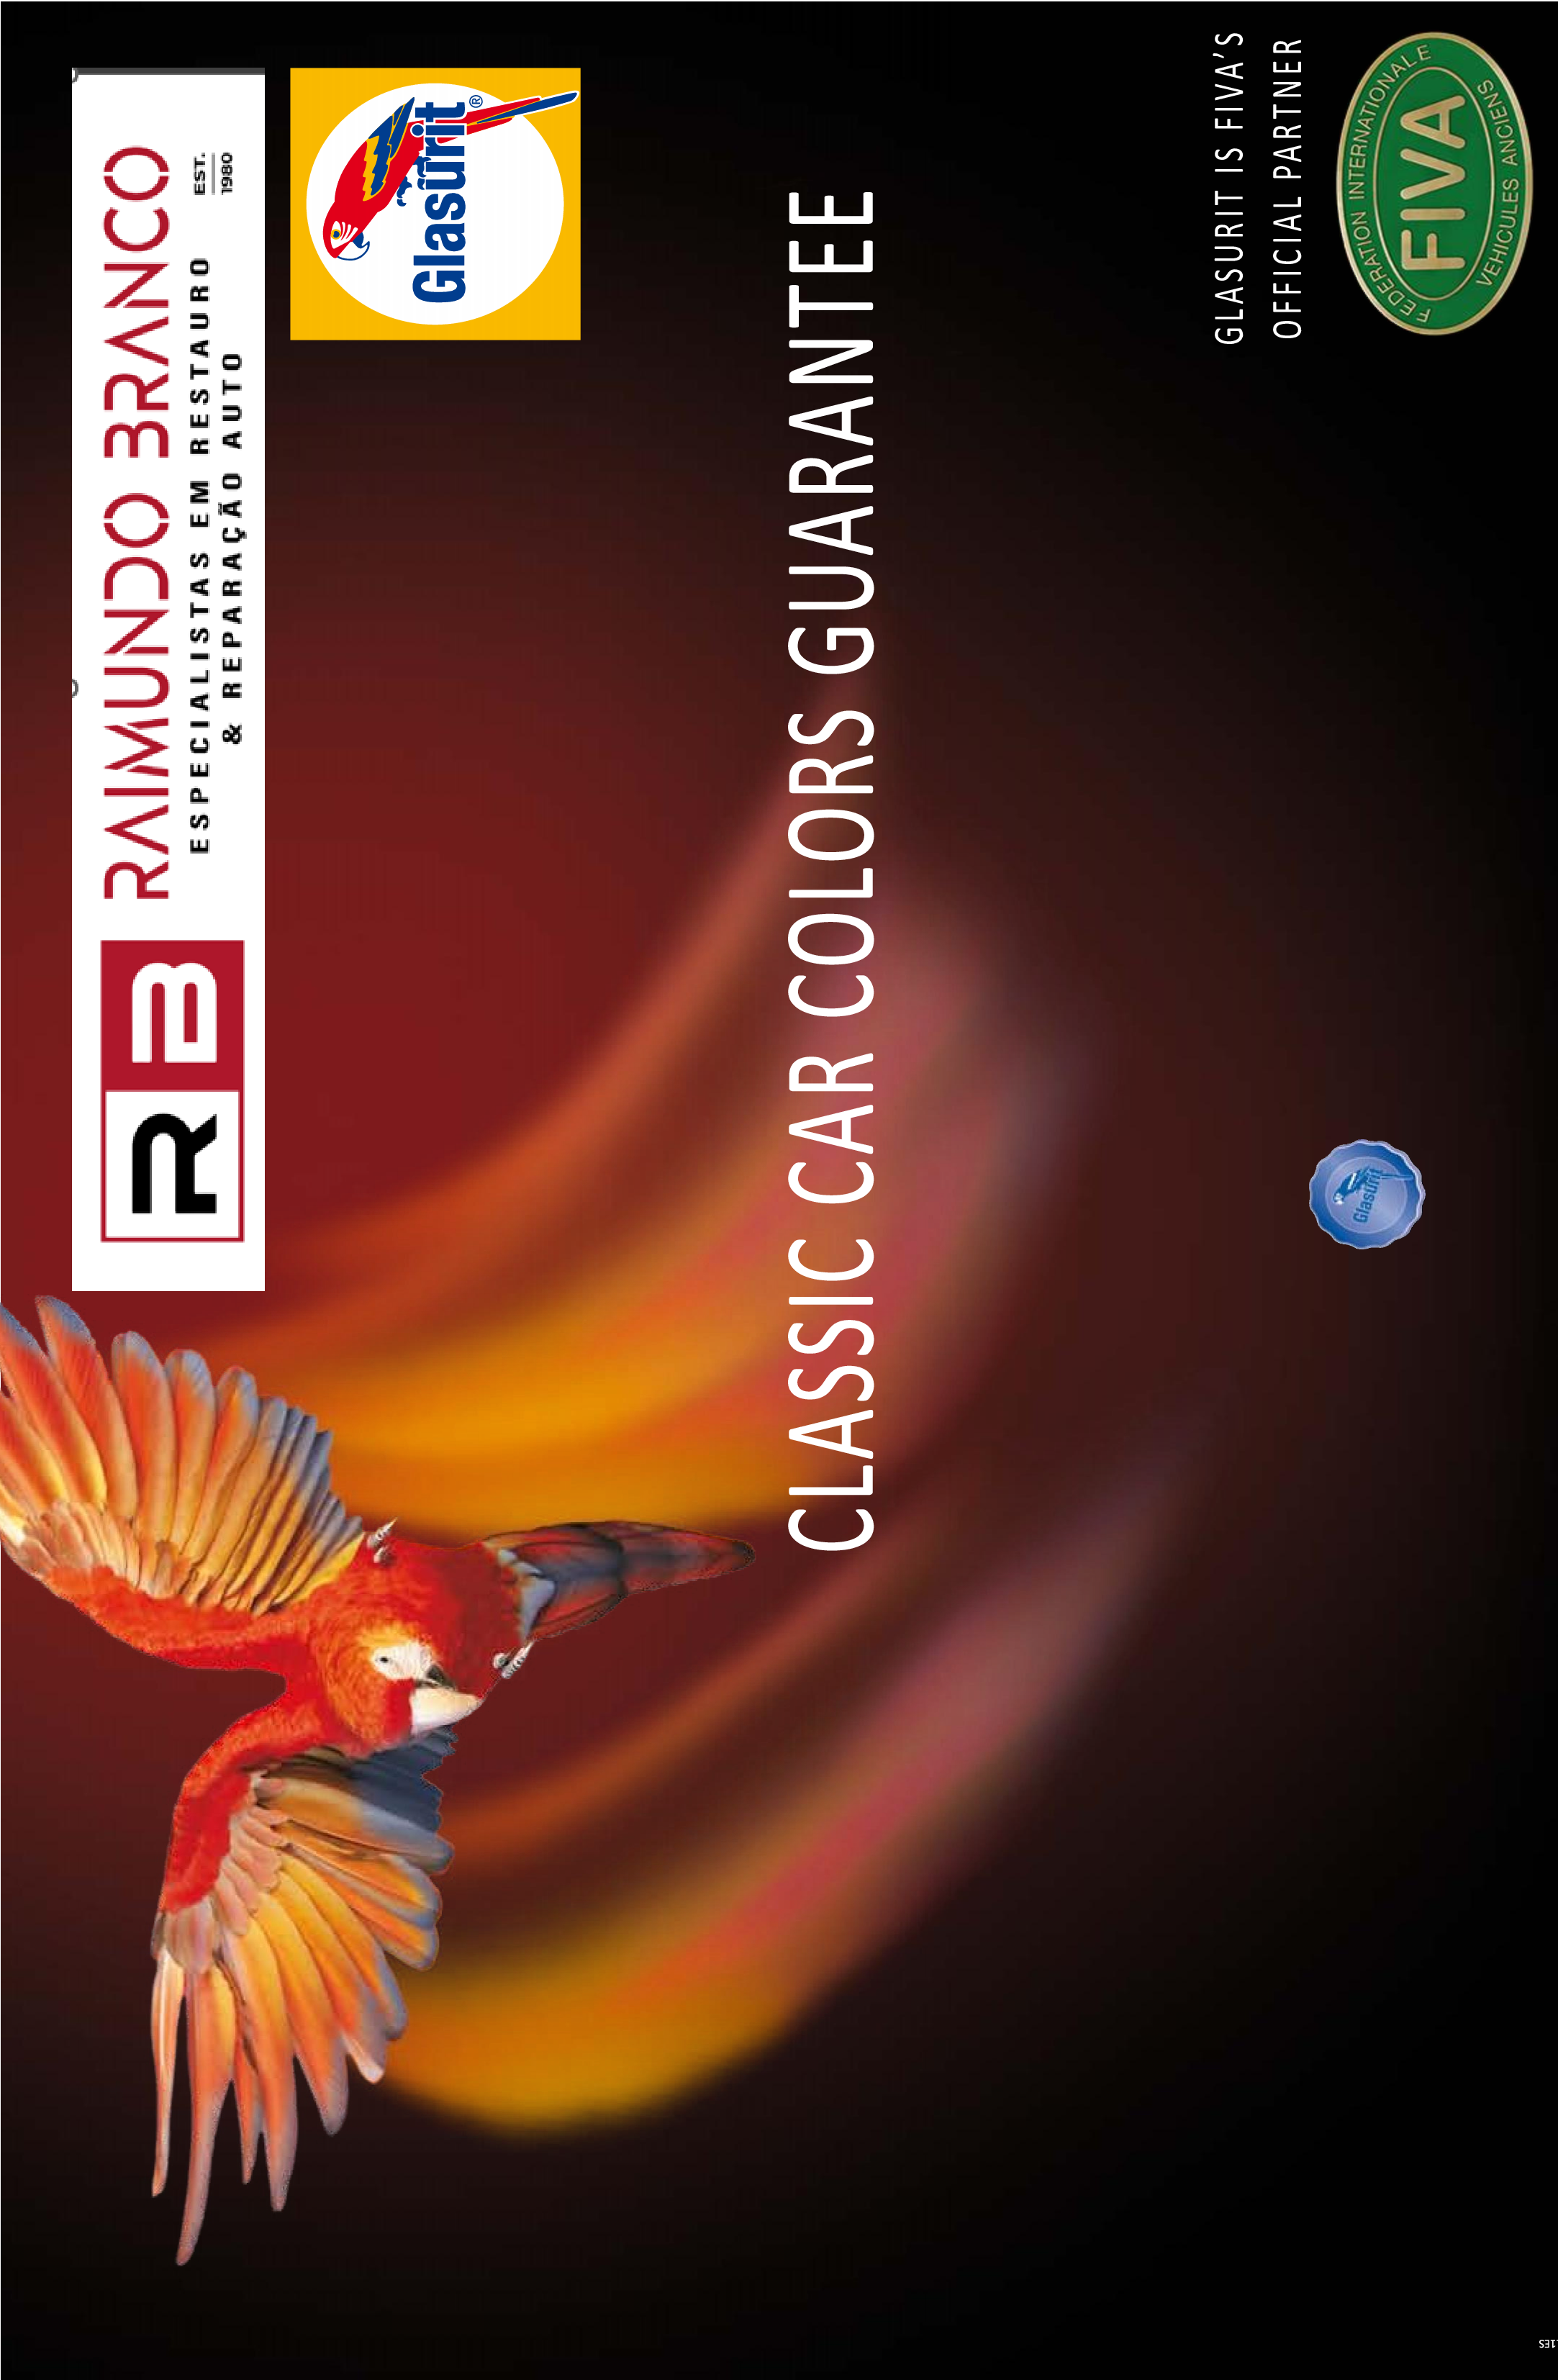
\includegraphics[width=\paperwidth,height=\paperheight]{logos/GlasuritGuaranteeBackground(rotated).png}}
}

\begin{landscape}

    \thispagestyle{empty}

    \begin{tikzpicture}[opacity=0, overlay]
        \node[fill=white, text=white, text opacity=1, inner sep=5pt, text width=0.8\paperwidth, align=center] at (6in, -4.5in) 
        {
            {\Huge Rolls Royce Corniche Silver Shadow (1976)}\\
            {\huge – DH 858 VR -}
        };
    \end{tikzpicture}

    \begin{tikzpicture}[opacity=0, overlay]
      \node[fill=white, text=white, text opacity=1, inner sep=5pt, text width=0.4\paperwidth, align=left] at (2, -6in) 
      {
            \textbf{COLOR REFERENCE}\\
            Record number: DH 858 VR\\
            %Record number: $\testee$\\
            Designation: WN HYUNDAI\\
            Technique: GLOSS\\
            Year: 1976
      };
    \end{tikzpicture}

\end{landscape}


\end{document}